%!TEX root = ../Pflichtenheft.tex


\chapter{Product overview}


\section{Production environment}
In the following, we describe the expected environment the system will be accessible in.
We differentiate between the \textbf{front-end}, i.e.\ the web interface and the \textbf{back-end}, i.e.\ the server component.

\subsection{Frontend}
The web interface of the system is designed for use in a modern web browser.
Explicitly supported are:
\begin{enumerate}
	\item \textit{Firefox}, stable releases from version \texttt{110.0} upwards.
	\item \textit{Google Chrome}, stable releases from version \texttt{120.0.0.0} upwards.
\end{enumerate}
Per~\ref{Q120}, support will be provided for \textit{Desktop}, \textit{Tablet} and \textit{Mobile} device sizes.

\subsection{Backend}
The server component of the system is designed for long and constant uptime. \newline
Deployment is intended to be performed via containerization techniques.
Explicitly supported is \textit{Docker} \footnote{https://www.docker.com/}, stable versions of major release \texttt{28} upwards. \newline
The host device needs access to a stable connection to the internet of at least \texttt{256} \hyperref[abr:Mbit/s]{Mbit/s} and latency of at most \texttt{100} ms. \newline
A domain or static IP needs to point towards the host machine the server is running on. \hyperref[abr:https]{HTTPS} encryption and certificates need to be provided externally and are not in the scope of this project. \newline
The host device must provide at least 4\hyperref[abr:GB]{GB} of memory and 16 \hyperref[abr:GB]{GB} of free storage to the system, to be distributed among the server and the utilized database

\section{Use-Cases}
The following provides a list of \textbf{use cases} of the app.
\textbf{Use cases} are used to list single actions that a user can perform when using the system.
Use cases specify the target that is intended by a user when performing an action and are used to broadly describe what the system can do.

\subsection{Account management}

\begin{figure}
\centering
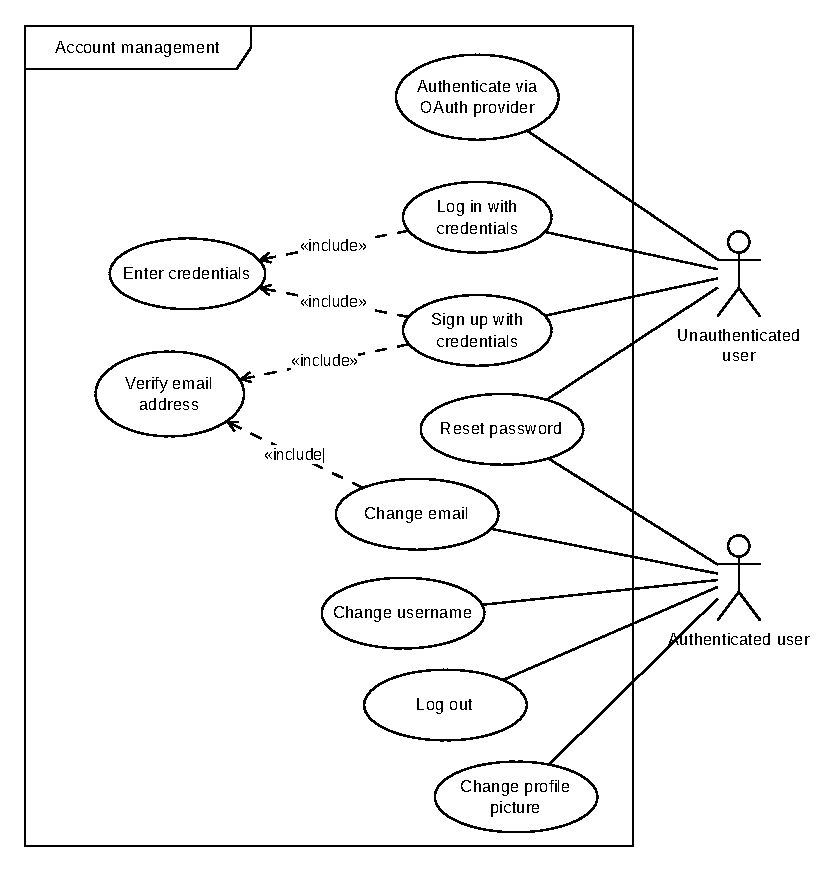
\includegraphics{figures/drawio/uc_account_management}
\caption{Use cases for managing the account.}
\label{fig:uc_account_management}
\end{figure}

Figure~\ref{fig:uc_account_management} shows the use cases that are related to account management and authorization of users. \newline
An \textbf{Authenticated} user is a user that is logged into an account and performs its actions in the context of that account.
An \textbf{Unauthenticated} user is a user that is not logged into an account. \newline
Both use cases \textbf{Sign up with credentials} and \textbf{Log in with credentials} require the user to \textbf{Enter credentials} for that specific account.
Furthermore, \textbf{Sign up with credentials} and \textbf{Change email} both result in the need for the user to \textbf{Verify the email address}.
Personal data change is performed with the use cases \textbf{Change username} and \textbf{Change profile picture}.
Additionally, authenticated users can \textbf{Log out} of the current account. \newline
Following, the use cases \textbf{Verify email address} (\ref{subsubsec:verify-email-address}), \textbf{Reset password} (\ref{subsubsec:reset-password}), and \textbf{Authenticate via \hyperref[def:oauth]{OAuth} provider} (\ref{subsubsec:authenticate-with-oauth}) are further expanded on.

\subsubsection{Verify email address}\label{subsubsec:verify-email-address}
\begin{figure}
	\centering
	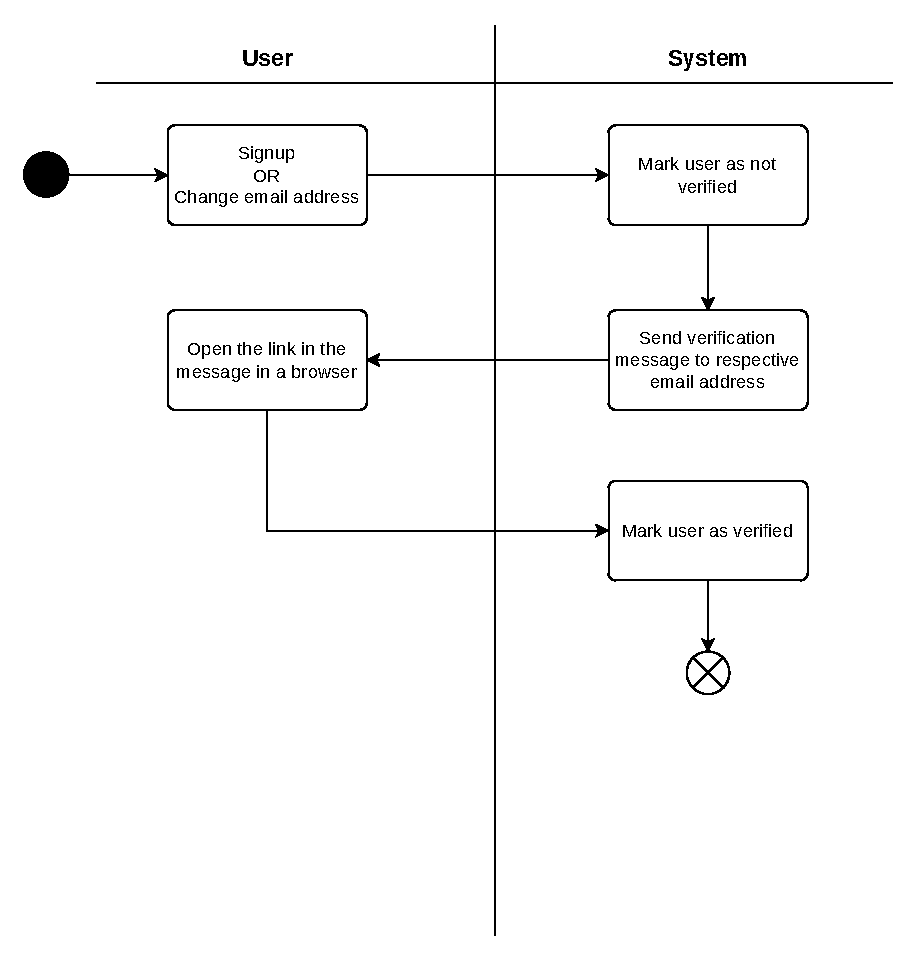
\includegraphics{figures/drawio/a_verify_email_address}
	\caption{Use case: Verify email address.}
	\label{fig:a_verify_email_address}
\end{figure}

Figure~\ref{fig:a_verify_email_address} shows the functions involved in performing the \textbf{Verify email address} use case. \newline
The use case is triggered either by a user signing up, or by changing the email address of their account.
The system sends a message to the new email address, which the user can use to verify their account.

\subsubsection{Reset password}\label{subsubsec:reset-password}
\begin{figure}
	\centering
	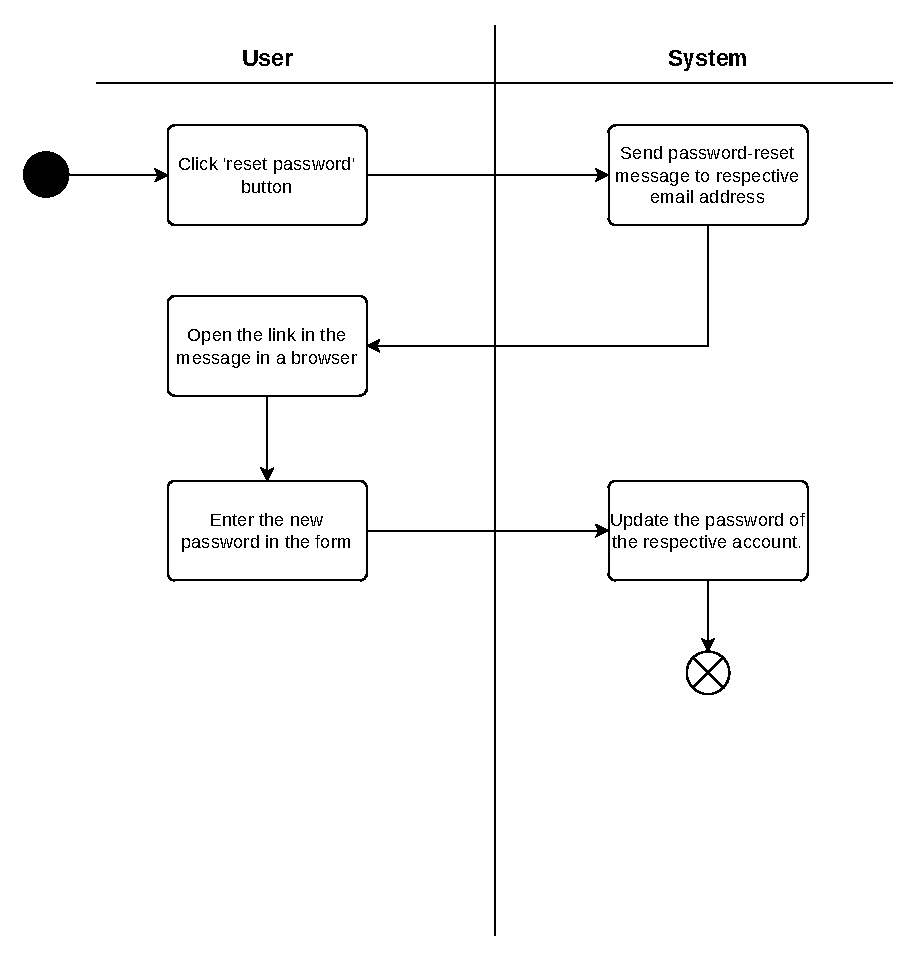
\includegraphics{figures/drawio/a_reset_password}
	\caption{Use case: Reset password.}
	\label{fig:a_reset_password}
\end{figure}

Figure~\ref{fig:a_reset_password} shows the functions involved in performing the \textbf{Reset password} use case. \newline
The use case is triggered actively by the user.
After that, the system sends a message to the user's email address, which contains a link where the user can enter the new password.
Finally, the user can authenticate with the new password.

\subsubsection{Authenticate via \hyperref[def:oauth]{OAuth} provider}\label{subsubsec:authenticate-with-oauth}
\begin{figure}
	\centering
	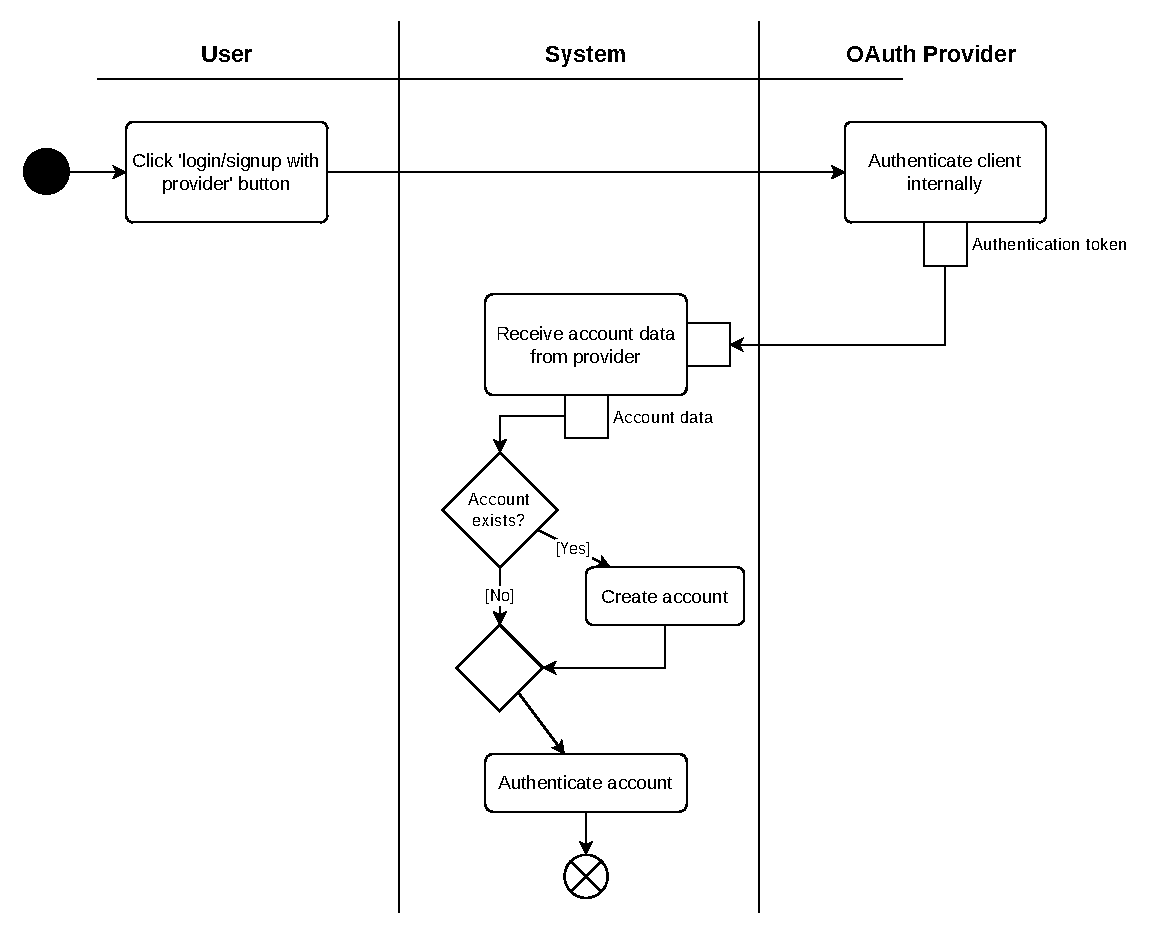
\includegraphics[width=\linewidth]{figures/drawio/a_auth_with_oauth}
	\caption{Use case: Authenticate via \hyperref[def:oauth]{OAuth} provider.}
	\label{fig:a_auth_with_oauth}
\end{figure}

Figure~\ref{fig:a_auth_with_oauth} shows the functions involved in performing the \textbf{Authenticate via \hyperref[def:oauth]{OAuth} provider} use case. \newline
This use case is triggered by a user selecting the \textit{\hyperref[def:oauth]{OAuth}} provider on the log-in/signup screen.
The authentication is handled by the provider.
This could be via credentials, using available cookies or other internal mechanisms.
After the internal authentication was performed, an access token is provided to the \textbf{CodeX} system, which it uses to connect the external account to a \textbf{CodeX} account, or create a new one if it doesn't yet exist.

\subsection{Conversations}

\begin{figure}
	\centering
	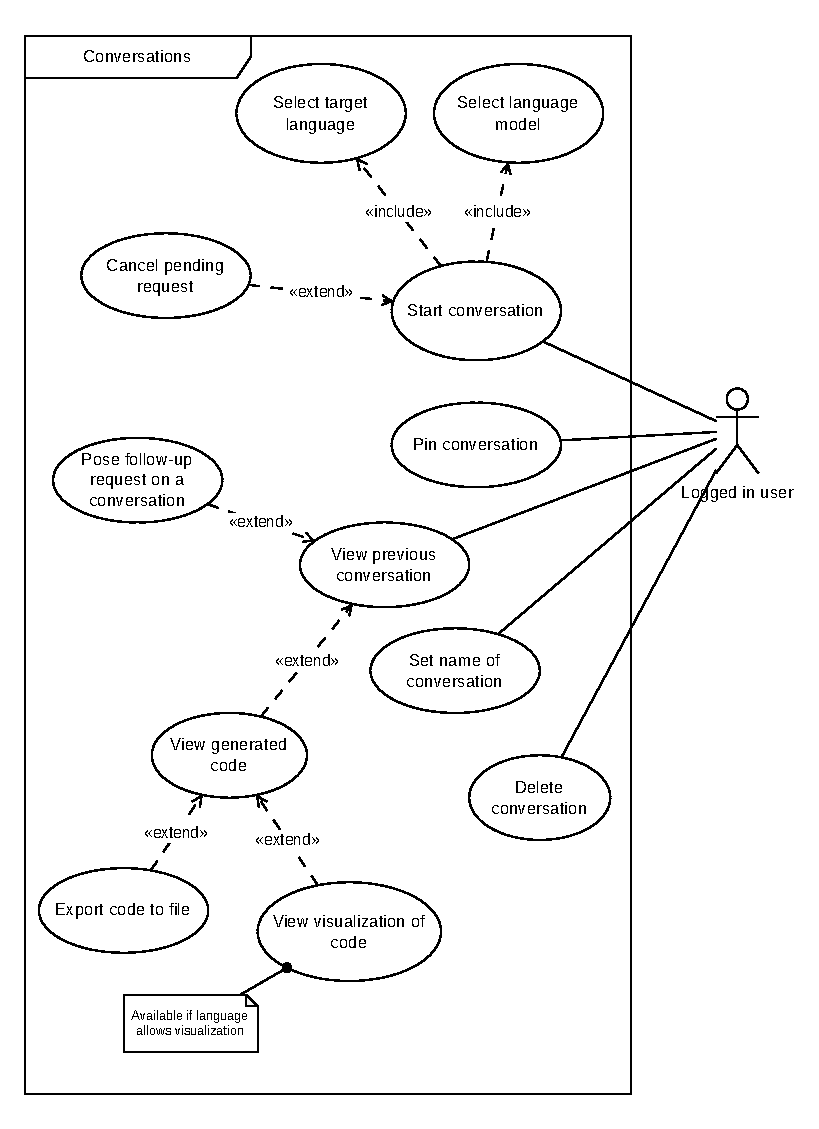
\includegraphics{figures/drawio/uc_conversations}
	\caption{Use cases for interacting with conversations.}
	\label{fig:uc_conversations}
\end{figure}

Figure~\ref{fig:uc_conversations} shows the use cases that describe how a user can interact with single or multiple conversations. \newline
In the list of all conversations, single ones can be \textbf{pinned to the top}, \textbf{assigned a name} or be \textbf{deleted}.
Users can also \textbf{View previous conversations} and \textbf{Pose follow-up questions on a conversation}.
When a request is pending, it can be \textbf{canceled}.
For an existing conversation, the user can \textbf{View the generated code} and optionally \textbf{Export the code to a file} or \textbf{View a visualization of the code}, if supported. \newline
The use-case \textbf{Start conversation} is further expanded on in \ref{subsubsec:start-conversation}.

\subsubsection{Start conversation}\label{subsubsec:start-conversation}
\begin{figure}
	\centering
	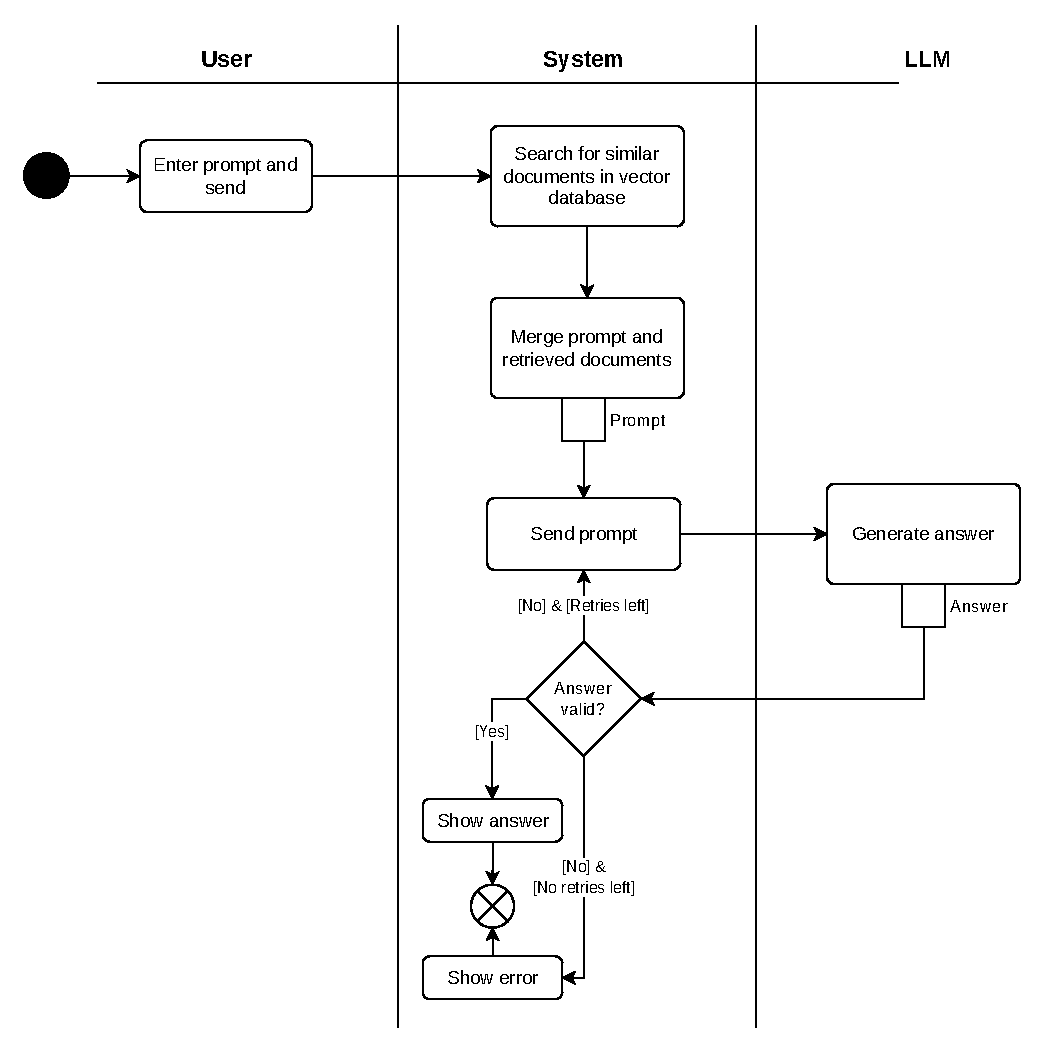
\includegraphics[width=\linewidth]{figures/drawio/a_start_conversation}
	\caption{Use case: Start conversation.}
	\label{fig:a_start_conversation}
\end{figure}

Figure~\ref{fig:a_start_conversation} shows the functions involved in performing the \textbf{Start conversation} use case. \newline
This use case is triggered by a user entering a prompt and sending it.
The system will associate the prompt with a list of documents retrieved from the vector database and merge it with the original prompt of the user.
This combined prompt is sent to the \textit{\hyperref[abr:LLM]{LLM}}, which in turn generates a response.
Depending on the target language, this answer is validated.
If the validation fails, the system retries the request several times and shows a response to the user.

\subsection{Admin Panel}

\begin{figure}
	\centering
	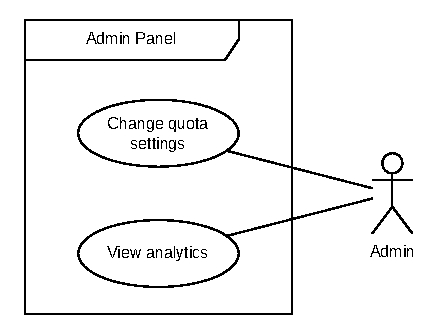
\includegraphics{figures/drawio/uc_admin_panel}
	\caption{Use cases for admin actions.}
	\label{fig:uc-admin-panel}
\end{figure}

Figure~\ref{fig:uc-admin-panel} shows the use cases that describe the actions that are specific to admins. \newline
Admins can \textbf{Change quota settings}, i.e.\ enabling/disabling quotas for specific roles and set the maximum number of requests.
Additionally, admins can view analytic data. \newline

\subsection{Settings}
\begin{figure}
	\centering
	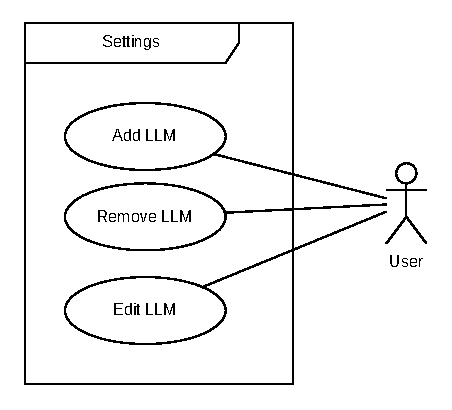
\includegraphics{figures/drawio/uc_settings}
	\caption{Use cases for settings.}
	\label{fig:uc-settings}
\end{figure}

Figure~\ref{fig:uc-settings} shows the use cases that describe the actions that can be performed in the settings section. \newline
Users can \textbf{add}, \textbf{edit} and \textbf{remove} \textit{\hyperref[abr:LLM]{LLM}} models.

\subsection{Miscellaneous}

\begin{figure}
	\centering
	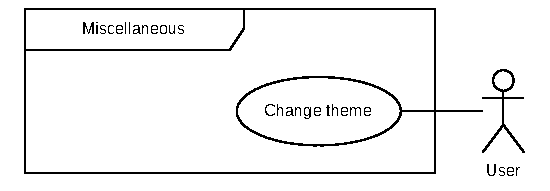
\includegraphics{figures/drawio/uc_miscellaneous}
	\caption{Miscellaneous use cases.}
	\label{fig:uc_miscellaneous}
\end{figure}

Figure~\ref{fig:uc_miscellaneous} contains miscellaneous use cases that don't fit in other categories. \newline
\textbf{Change theme} refers to the action of a user being able to toggle the color theme of the user interface between light and dark mode.